\section{Test Description and Success Criteria}

The unit test for the thruster\_dynamics module is located in:\\

\noindent
{\tt simulation/dynamics/Thrusters/$\_$UnitTest/unit$\_$ThrusterDynamicsUnit.py} \\

\subsection{Test inputs}

The thruster inputs that were used are:

\begin{itemize}
\item Earth's gravity on surface : $g=9.80665$ m s$^{-2}$ 
\item The specific impulse: $I_{sp} = 266.7$s. As seen previously, we use the definition of specific impulse defined by:

\begin{equation*}
F_{\mathrm{thrust}} = g_0 \dot{m} I_{sp}
\end{equation*}

This has the units of seconds, and uses the earths gravitational constant. It represents a thrusters potential to deliver force per mass flow rate. 
\item The maximum thrust: $F_{\mathrm{max}} = 1.0$ N

The scaling factor yielding the thrust.
\item The minimum On time: $t_{\mathrm{min}} = 0.006$s

The minimum time that the thruster can be fired.

\item The maximum swirl torque: $T_{\mathrm{maxSwirl}} = 0.5$ Nm
\end{itemize}

\subsection{Test sections}

\noindent This unit test is designed to functionally test the simulation model 
outputs as well as get complete code path coverage. 
The test design is broken 
up into several parts, and the mass flow rate is tested at each of these subtests. :\\
\begin{enumerate}
\item{\underline{Instantaneous On/Off Factor:} The thrusters are fired with an 
  instantaneous ramp to ensure that the firing is correct. This gives us a base case.}
\item{\underline{Short Instantaneous Firing:} A "short" firing that still respects the 
  rule of thumb above is fired to ensure that it is still correct.}
 \item{\underline{Short Instantaneous Firing with faster test rate:} A "short" firing that still respects the 
  rule of thumb above but with a faster test rate to see the jump.}
 \item{\underline{Instantaneous On/Off Factor with faster test rate:} The thrusters are fired with an 
  instantaneous ramp to ensure that the firing is correct given a different test rate. This shouldn't modify the physics.}
 \item{\underline{Thruster Angle Test:} The output forces/torques from the simulation 
  are checked with a thruster pointing in a different direction.}
   \item{\underline{Thruster Position Test:} The output forces/torques from the simulation 
  are checked with a thruster in a different position.}
   \item{\underline{Thruster Number Test:} The output forces/torques from the simulation 
  are checked with two thruster in different positions, with different angles.}
\item{\underline{Ramp On/Ramp Off Firing:} A set of ramps are set for the thruster to ensure 
  that the ramp configuration is respected during a ramped firing.}
  \item{\underline{Short ramped firing:} A thruster is fired for less than the amount of time it 
   takes to reach the end of its ramp.}
\item{\underline{Ramp On/Ramp Off Firing with faster test rate:} A set of ramps are set for the thruster to ensure 
  that the ramp configuration is respected during a ramped firing with different test rate.}
\item{\underline{Cutoff firing:} A thruster is commanded off (zero firing time) in the middle 
   of its ramp up to ensure that it correctly cuts off the current firing}
\item{\underline{Ramp down firing:} A thruster is fired during the middle of its ramp down 
   to ensure that it picks up at that point in its ramp-up curve and reaches 
   steady state correctly.}
\item{\underline{Swirl torque:} A thruster is fired with swirl torque active to make sure that the additional torque about the thrust axis is accounted for.}
\end{enumerate}

These scenarios create a set of different runs. These are run in the same test using pytest parameters. Therefore 13 different parameter sets were created to cover all of the listed parts.

\subsection{Test success criteria}

This thrusters test is considered successful if, for each of the scenarios, the output data matches exactly the truth data that is computed in python. This means that at every time step, the thrust is the one that is expected down to near machine precision ($\epsilon = 10^{-9}$). 

This leaves no slack for uncertainty in the thrusters module.



\section{Test Parameters}


In order to have a rigorous automated test, we have to predict the forces and torques that will apply on the spacecraft. We use the following equations to compute the thrust at each time step. We call $\alpha$ the angle in which the thruster is pointing, $\bm r = r \hat{\bm e_r}= \left(r_x, r_y, r_z \right)$ it's position vector in the body frame, 

\begin{enumerate}
	
	\item{\underline{Mass flow rate}}: 
	
	We compute the mass flow rate using the following equation:
	
	\begin{equation}
	\dot{m} = \frac{F}{g I_{sp}}
	\end{equation}
	
	Since we are using constant $I_{sp}$, thrust, and $g$ is constant, this is the same value throughout the tests. $\dot{m}$ is therefore either zero (when the thruster is not firing) or set to the previous value. 
	
	\item{\underline{With one thruster}}: The forces are simply the projections of the thrust force on the axes of interest. The torque along $x$ is the arm along $z$ times the projection of the force along $y$, the torque along $z$ is the arm along $x$ times the projection of the force along $y$, the torque along $z$ is the arm along $x$ times the projection of the force along $y$. 
	
	\begin{align}
		\leftexp{B}{\bm F} =\leftexp{B}{\begin{pmatrix} F_x, & F_y & F_z \end{pmatrix}}^T&\hspace{1cm} \leftexp{B}{\bm T} =\leftexp{B}{\bm r} \times \leftexp{B}{\bm F} +  \leftexp{B}{\bm T}_{\mathrm{swirl}}\\
	\end{align}
	
	
	\item{\underline{With two thrusters}}: By giving indices $1$ and $2$ for each of the thrusters, we just need to add the Forces and torques defined above to get the total Forces and Torques:
	
	\begin{align}
		\leftexp{B}{\bm F} = \leftexp{B}{\bm F_1}  + \leftexp{B}{\bm F_2} &\hspace{1cm} \leftexp{B}{\bm T} = \leftexp{B}{\bm T_1}  + \leftexp{B}{\bm T_2} \\ 
	\end{align}
	
	\item{\underline{With ramps thruster}}: When the thrusters now ramp up and down, we create a normalized ramp function $\rho$. An example is given in \ref{fig:Ramp_function} in the case of a cutoff fire and renewed fire. \par
	
	\begin{figure}[htbp]\centerline{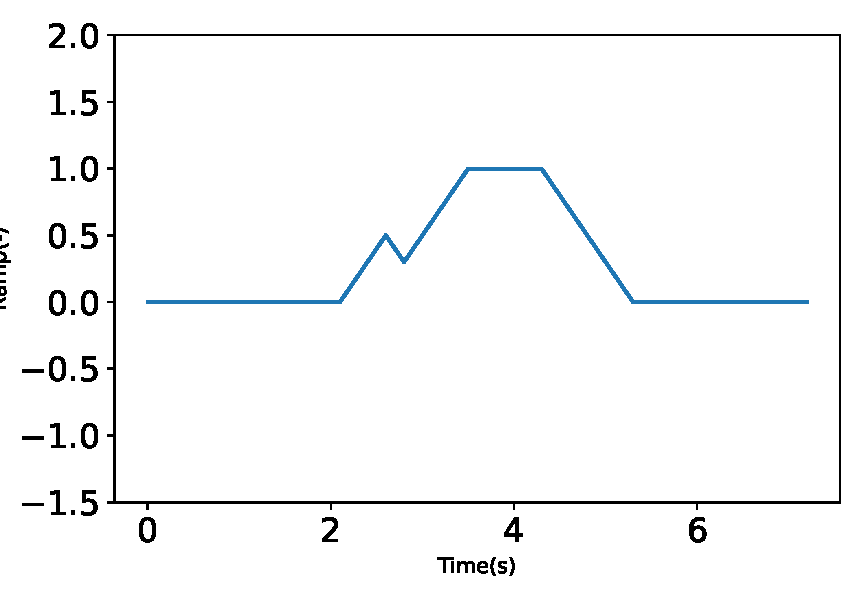
\includegraphics[width=0.8\textwidth]{AutoTeX/Ramp_function}}\caption{Example of ramp function}\label{fig:Ramp_function}\end{figure}
	
	We then prolong the force and torque end times as a function of the ramp slope, and multiply the initial functions by this ramping function:
	
	\begin{align}
		\tilde{\bm F} = \rho \bm F &\hspace{1cm} \tilde{\bm T} =\rho \bm T  \\ 
	\end{align}
	
\end{enumerate}



\section{Test Results}

\subsection{Pass/Fail}

\begin{center}
	\begin{tabular}{|c|c|c|}
		\hline
		Parameter Sets & Test Result & Error Tolerance \\ \hline \hline
		1  &\textcolor{ForestGreen}{PASSED} & $10^{-9}$ \\ \hline
		2  &\textcolor{ForestGreen}{PASSED} & $10^{-9}$ \\ \hline
		3  &\textcolor{ForestGreen}{PASSED} & $10^{-9}$ \\ \hline
		4  &\textcolor{ForestGreen}{PASSED}& $10^{-9}$ \\ \hline
		5  &\textcolor{ForestGreen}{PASSED}& $10^{-9}$ \\ \hline
		6  & \textcolor{ForestGreen}{PASSED} & $10^{-9}$ \\ \hline
		7  &\textcolor{ForestGreen}{PASSED}& $10^{-9}$ \\ \hline
		8  &\textcolor{ForestGreen}{PASSED} & $10^{-9}$ \\ \hline
		9  &\textcolor{ForestGreen}{PASSED} & $10^{-9}$ \\ \hline
		10  &\textcolor{ForestGreen}{PASSED}& $10^{-9}$ \\ \hline
		11  &\textcolor{ForestGreen}{PASSED} & $10^{-9}$ \\ \hline
		12  &\textcolor{ForestGreen}{PASSED} & $10^{-9}$ \\ 
		\hline
		
	\end{tabular}
\end{center}

\begin{enumerate}
	\item{\underline{ Instantaneous On/Off Factor}:} 
	
	The thruster is set at 30$^\circ$ off the x-axis 15$^\circ$ off the z-axis, in the position $\bm r = \left(1.125,0.5,2.0\right)$. The test is launched using 1 thruster, for 5.0 seconds. The test rate is 10 steps per second
	
	Figures \ref{fig:Force_1Thrusters_5s_30deg_Loc2_Rate10} and \ref{fig:Torque_1Thrusters_5s_30deg_Loc2_Rate10} show the force and torque behaviors (respectfully) for the thruster unit test.
	
	\begin{figure}[htbp]\centerline{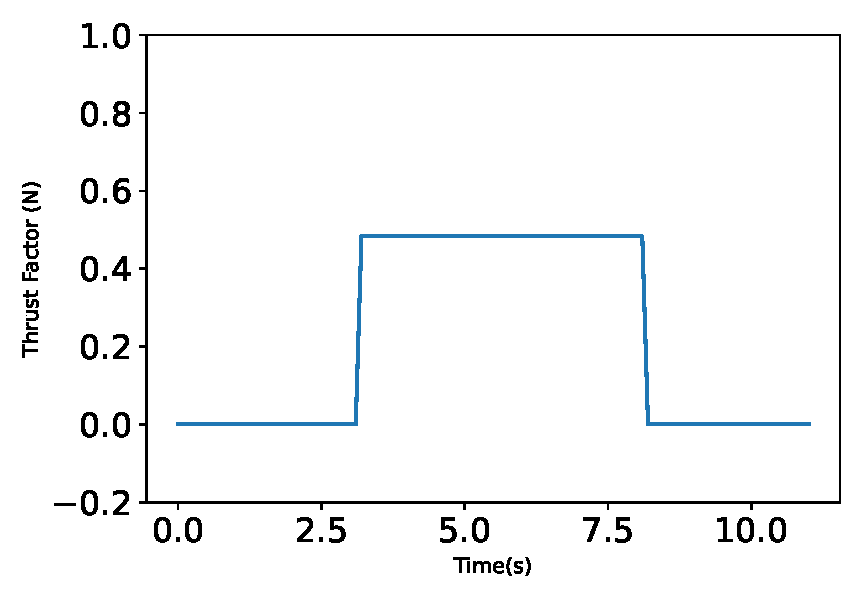
\includegraphics[width=0.8\textwidth]{AutoTeX/Force_1Thrusters_5s_30deg_Loc2_Rate10}}\caption{Force on Y with 1 thrusters, for 5 sec at 30 deg Rate10}\label{fig:Force_1Thrusters_5s_30deg_Loc2_Rate10}\end{figure}
	\begin{figure}[htbp]\centerline{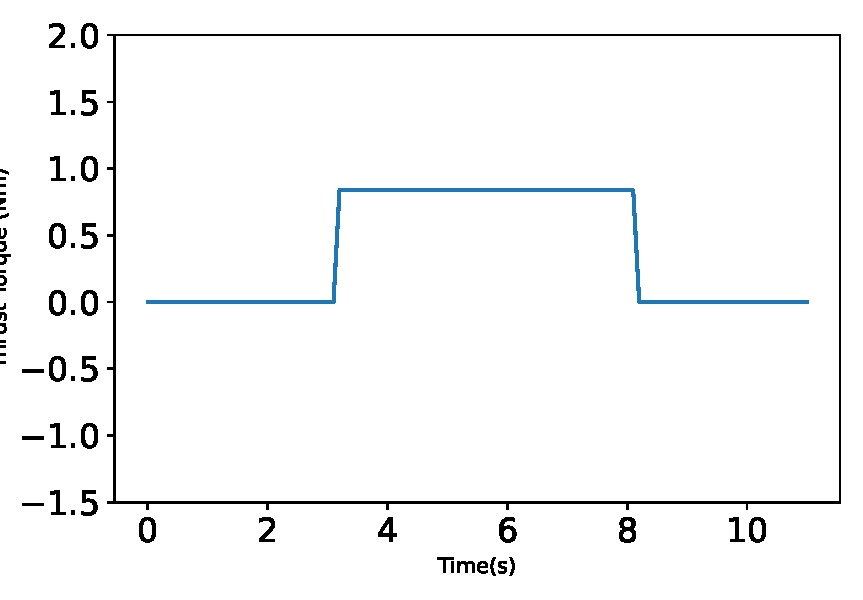
\includegraphics[width=0.8\textwidth]{AutoTeX/Torque_1Thrusters_5s_30deg_Loc2_Rate10}}\caption{Torque on X with 1 thrusters, for 5 sec at 30 deg Rate10}\label{fig:Torque_1Thrusters_5s_30deg_Loc2_Rate10}\end{figure}
	\begin{figure}[htbp]\centerline{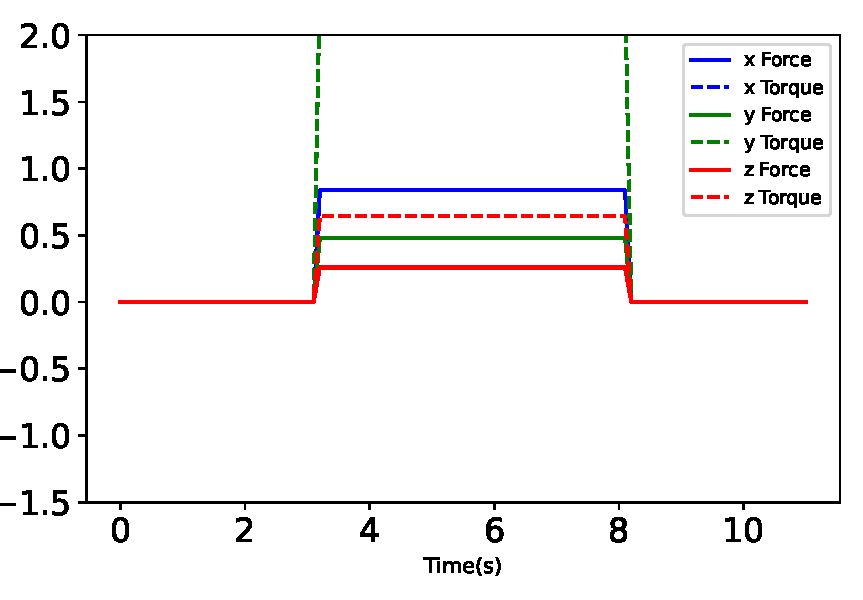
\includegraphics[width=0.8\textwidth]{AutoTeX/1Thrusters_5s_30deg_Loc2_Rate10}}\caption{All Forces and Torques 1 thrusters, for 5 sec at 30 deg Rate10}\label{fig:1Thrusters_5s_30deg_Loc2_Rate10}\end{figure}
	
	As Figure \ref{fig:1Thrusters_5s_30deg_Loc2_Rate10} shows, the desired behavior is captured exactly for each 
	firing in the test for all of the forces and torques. This is validated by the exact same predicted and simulated thrust arrays.  
	
	\item{\underline{Short Instantaneous Firing: }}
	
	The thruster is set at 30$^\circ$ off the x-axis 15$^\circ$ off the z-axis, in the position $\bm r = \left(1.125,0.5,2.0\right)$. The test is launched using 1 thruster, for 0.1 seconds. The test rate is 10 steps per second
	
	Figure \ref{fig:Force_1Thrusters_0s_30deg_Loc2_Rate10} shows the force behavior given this short input. We see that the test rate begin small next to the thrust duration, doesn't capture the jump quite well.
	
	\begin{figure}[htbp]\centerline{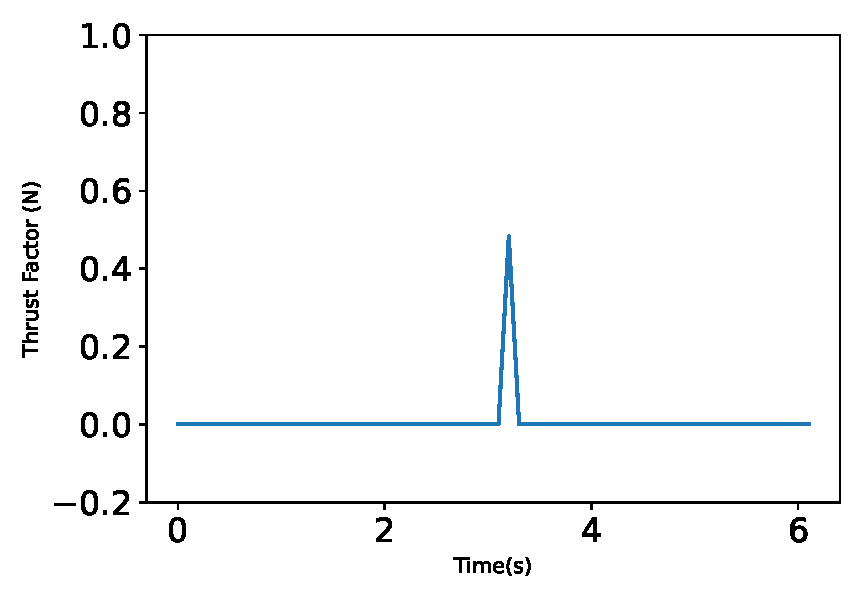
\includegraphics[width=0.8\textwidth]{AutoTeX/Force_1Thrusters_0s_30deg_Loc2_Rate10}}\caption{Force on Y with 1 thrusters, for 0 sec at 30 deg Rate10}\label{fig:Force_1Thrusters_0s_30deg_Loc2_Rate10}\end{figure}
	\begin{figure}[htbp]\centerline{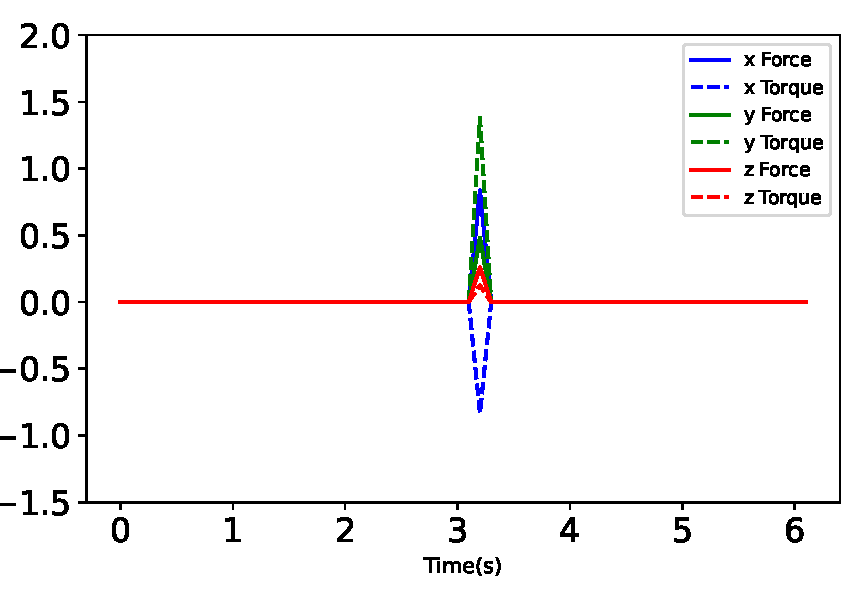
\includegraphics[width=0.8\textwidth]{AutoTeX/1Thrusters_0s_30deg_Loc2_Rate10}}\caption{All Forces and Torques 1 thrusters, for 0 sec at 30 deg Rate10}\label{fig:1Thrusters_0s_30deg_Loc2_Rate10}\end{figure}
	
	As Figure \ref{fig:1Thrusters_0s_30deg_Loc2_Rate10} shows, the desired behavior is captured exactly for each 
	firing in the test for all of the forces and torques. Despite the lower test rate, the forces and torques behave appropriately. This is validated by the exact same predicted and simulated thrust arrays.
	
	\item{\underline{Short Instantaneous Firing with faster test rate: }}
	
	The thruster is set at 30$^\circ$ off the x-axis 15$^\circ$ off the z-axis, in the position $\bm r = \left(1.125,0.5,2.0\right)$. The test is launched using 1 thruster, for 0.1 seconds. The test rate is 1000 steps per second
	
	Figure \ref{fig:Force_1Thrusters_0s_30deg_Loc2_Rate1000} shows the force behavior given the same short input as previously. We now see that the jump is well resolved.
	
	\begin{figure}[htbp]\centerline{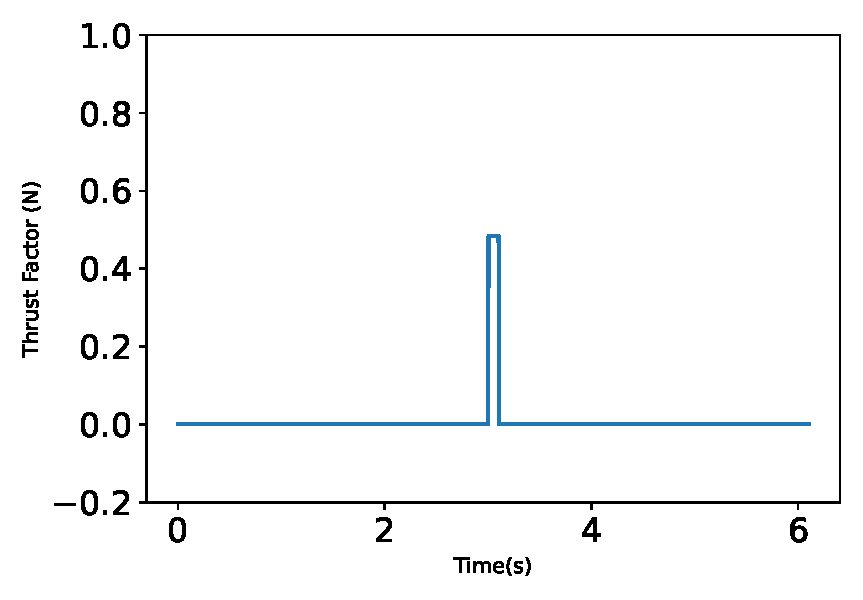
\includegraphics[width=0.8\textwidth]{AutoTeX/Force_1Thrusters_0s_30deg_Loc2_Rate1000}}\caption{Force on Y with 1 thrusters, for 0 sec at 30 deg Rate1000}\label{fig:Force_1Thrusters_0s_30deg_Loc2_Rate1000}\end{figure}
	\begin{figure}[htbp]\centerline{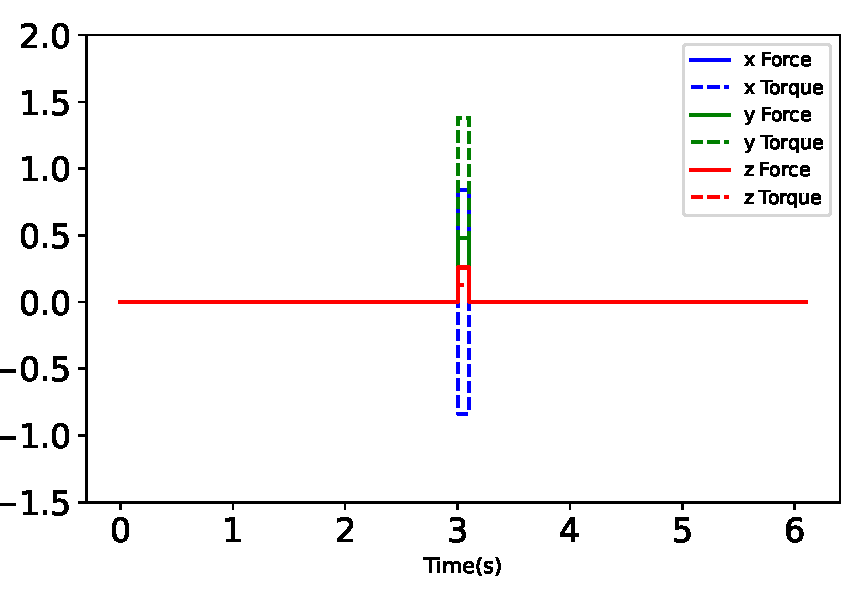
\includegraphics[width=0.8\textwidth]{AutoTeX/1Thrusters_0s_30deg_Loc2_Rate1000}}\caption{All Forces and Torques 1 thrusters, for 0 sec at 30 deg Rate1000}\label{fig:1Thrusters_0s_30deg_Loc2_Rate1000}\end{figure}
	
	As Figure \ref{fig:1Thrusters_0s_30deg_Loc2_Rate1000} shows, the desired behavior is captured exactly for each 
	firing in the test for all of the forces and torques. This is validated by the exact same predicted and simulated thrust arrays. 
	
	\item{\underline{Instantaneous On/Off Factor with faster test rate:} }
	
	The thruster is set at 30$^\circ$ off the x-axis 15$^\circ$ off the z-axis, in the position $\bm r = \left(1.125,0.5,2.0\right)$. The test is launched using 1 thruster, for 5.0 seconds. The test rate is 100 steps per second
	
	The thrust command given is now 5 seconds long, as in the base test. The difference is that the test rate is now augmented in order to guarantee that it does not affect the test.
	
	\begin{figure}[htbp]\centerline{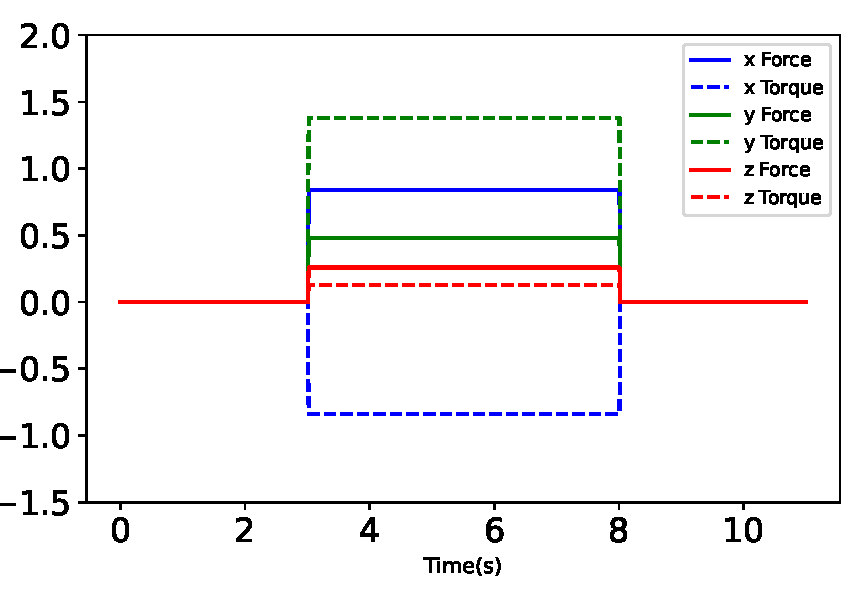
\includegraphics[width=0.8\textwidth]{AutoTeX/1Thrusters_5s_30deg_Loc2_Rate100}}\caption{All Forces and Torques 1 thrusters, for 5 sec at 30 deg Rate100}\label{fig:1Thrusters_5s_30deg_Loc2_Rate100}\end{figure}
	
	As Figure \ref{fig:1Thrusters_5s_30deg_Loc2_Rate100} shows, the desired behavior is captured exactly for each 
	firing in the test for all of the forces and torques. This is validated by the exact same predicted and simulated thrust arrays. 
	
	\item{\underline{Thruster Angle Test:}}
	
	The thruster is set at 10$^\circ$ off the x-axis 35$^\circ$ off the z-axis, in the position $\bm r = \left(1.125,0.5,2.0\right)$. The test is launched using 1 thruster, for 5.0 seconds. The test rate is 10 steps per second
	
	The test now shows that the simulation still behaves with different thruster orientations.
	
	\begin{figure}[htbp]\centerline{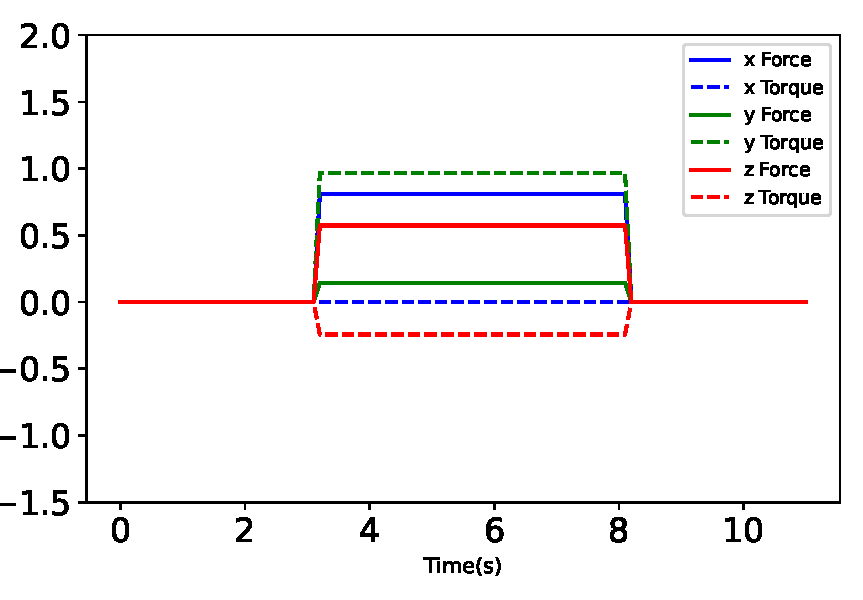
\includegraphics[width=0.8\textwidth]{AutoTeX/1Thrusters_5s_10deg_Loc2_Rate10}}\caption{All Forces and Torques 1 thrusters, for 5 sec at 10 deg Rate10}\label{fig:1Thrusters_5s_10deg_Loc2_Rate10}\end{figure}
	
	As Figure \ref{fig:1Thrusters_5s_10deg_Loc2_Rate10} shows, the desired behavior is captured exactly for each 
	firing in the test for all of the forces and torques. This is validated by the exact same predicted and simulated thrust arrays. 
	
	
	\item{\underline{Thruster Position Test:} }
	
	The thruster is set at 30$^\circ$ off the x-axis 15$^\circ$ off the z-axis, in the position $\bm r = \left(1.0,1.5,0.0\right)$. The test is launched using 1 thruster, for 5.0 seconds. The test rate is 10 steps per second
	
	This test shows that different locations still give correct values for forces and torques.
	
	\begin{figure}[htbp]\centerline{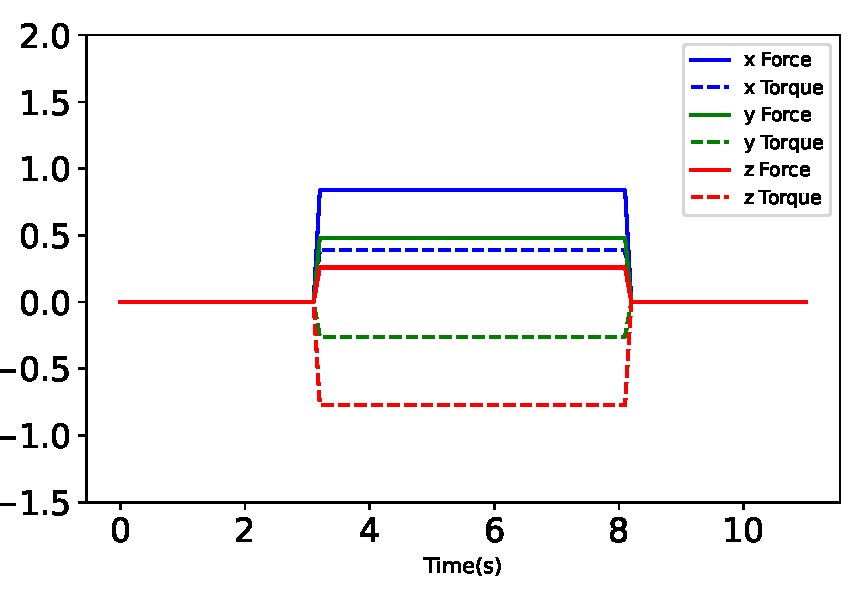
\includegraphics[width=0.8\textwidth]{AutoTeX/1Thrusters_5s_30deg_Loc0_Rate10}}\caption{All Forces and Torques 1 thrusters, for 5 sec at 30 deg Rate10}\label{fig:1Thrusters_5s_30deg_Loc0_Rate10}\end{figure}
	
	As Figure \ref{fig:1Thrusters_5s_30deg_Loc0_Rate10} shows, the desired behavior is captured exactly for each 
	firing in the test for all of the forces and torques. This is validated by the exact same predicted and simulated thrust arrays. 
	
	\item{\underline{Thruster Number Test:} }
	
	The first thruster is set at 30$^\circ$ off the x-axis 15$^\circ$ off the z-axis, in the position $\bm r = \left(1.125,0.5,2.0\right)$. The second thruster is set at 75$^\circ$ off the x-axis 60$^\circ$ off the z-axis, in the position $\bm r = \left(1.0,0.0,0.0\right)$. The test uses these 2 thrusters for 5.0 seconds. The test rate is 10 steps per second
	
	This test shows that the thruster model can incorporate several thrusters correctly. We add a second thruster and use the modified truth function for the forces and torques. These thrusters are not aligned and not in the same position, giving a general multi-thruster result.  
	
	\begin{figure}[htbp]\centerline{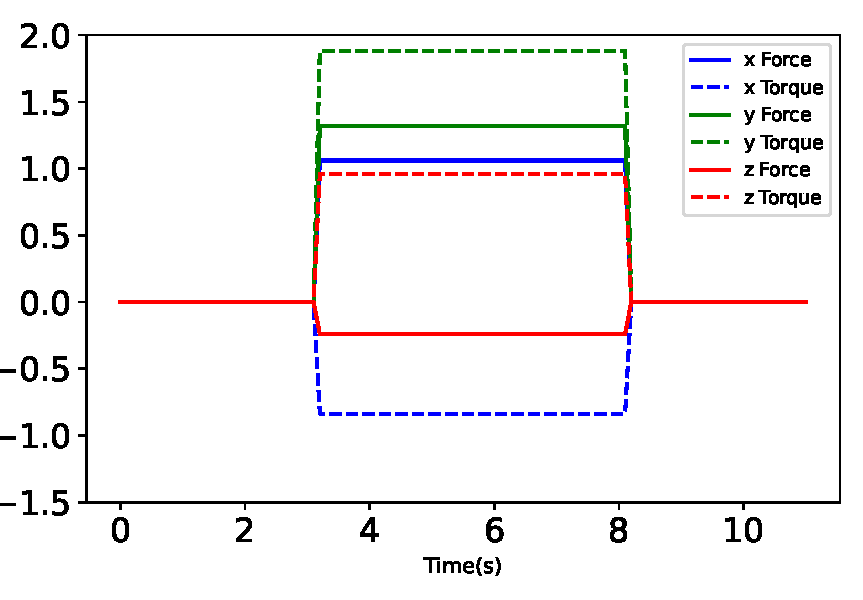
\includegraphics[width=0.8\textwidth]{AutoTeX/2Thrusters_5s_30deg_Loc2_Rate10}}\caption{All Forces and Torques 2 thrusters, for 5 sec at 30 deg Rate10}\label{fig:2Thrusters_5s_30deg_Loc2_Rate10}\end{figure}
	
	As Figure \ref{fig:2Thrusters_5s_30deg_Loc2_Rate10} shows, the desired behavior is captured exactly for each 
	firing in the test for all of the forces and torques. This is validated by the exact same predicted and simulated thrust arrays.  
	
	\item{\underline{Ramp On/Ramp Off Firing:} }
	
	We test the ramped thrust with 10 incremental steps. The single thruster is set at the default 30$^\circ$ off the x-axis 15$^\circ$ off the z-axis, at $\bm r = \left(1.125,0.5,2.0\right)$. The thrust is set for 5.0 seconds with a test rate of 10 steps per second. The Cutoff test is OFF
	
	This test now ramps the thrust up and down. We use a 10 step ramp that takes $0.1$s to climb and fall. This ramp time is slightly exaggerated in order to see the ramp clearly.      
	\begin{figure}[htbp]\centerline{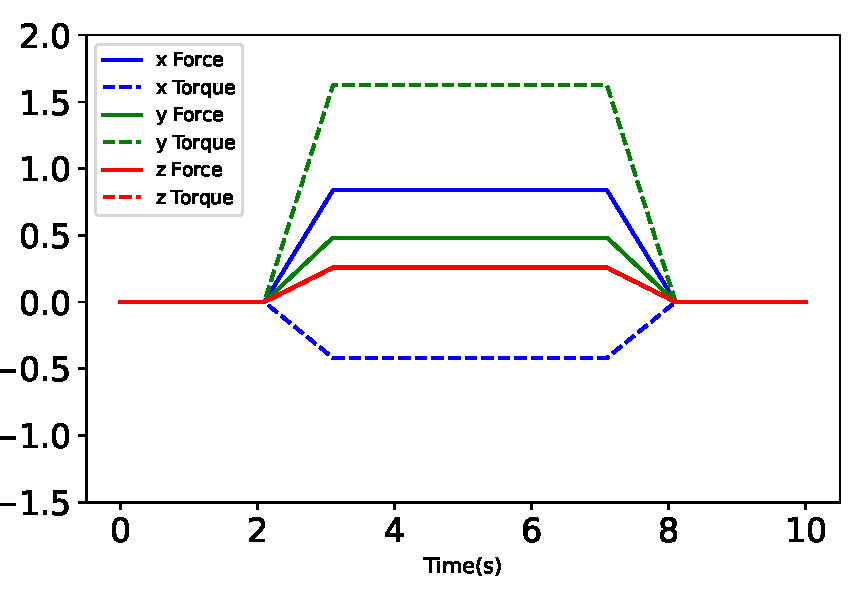
\includegraphics[width=0.8\textwidth]{AutoTeX/Ramp_10steps_CutoffOFF_5s_testRate10}}\caption{All Forces and Torques with 10 step Ramp, thrust for 5s. Cutoff OFF, testRate10}\label{fig:Ramp_10steps_CutoffOFF_5s_testRate10}\end{figure}
	
	As Figure \ref{fig:Ramp_10steps_CutoffOFF_5s_testRate10} shows, the desired behavior is captured exactly for each 
	firing in the test for all of the forces and torques. This is validated by the exact same predicted and simulated thrust arrays. 
	
	
	\item{\underline{Short ramped firing:} }
	
	We test the ramped thrust with 10 incremental steps. The single thruster is set at the default 30$^\circ$ off the x-axis 15$^\circ$ off the z-axis, at $\bm r = \left(1.125,0.5,2.0\right)$. The thrust is set for 0.5 seconds with a test rate of 10 steps per second. The Cutoff test is OFF
	
	Using the same ramp, the thruster fires for $0.5$s. We expect to see a climb and immediate fall of the thrust factor.
	
	\begin{figure}[htbp]\centerline{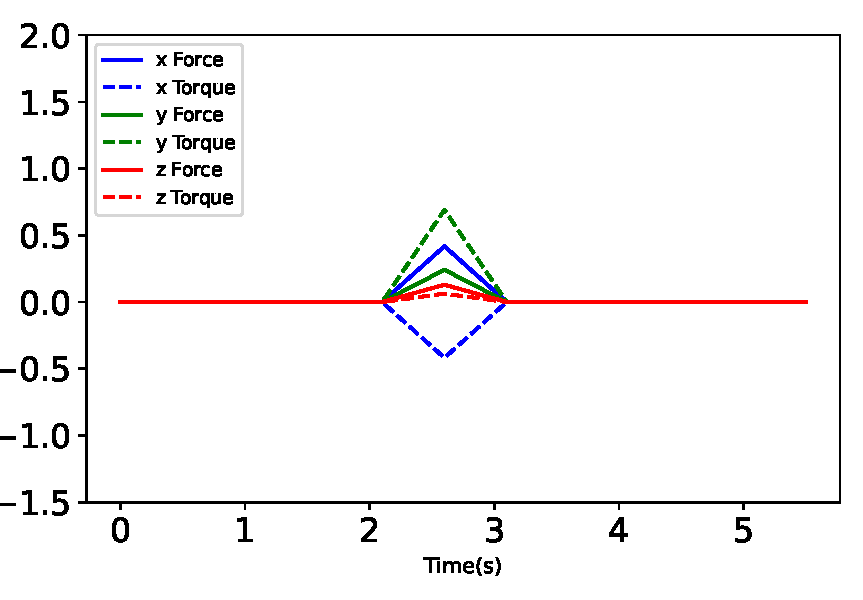
\includegraphics[width=0.8\textwidth]{AutoTeX/Ramp_10steps_CutoffOFF_0s_testRate10}}\caption{All Forces and Torques with 10 step Ramp, thrust for 0s. Cutoff OFF, testRate10}\label{fig:Ramp_10steps_CutoffOFF_0s_testRate10}\end{figure}
	
	As Figure \ref{fig:Ramp_10steps_CutoffOFF_0s_testRate10} shows, the desired behavior is captured exactly for each 
	firing in the test for all of the forces and torques. This is validated by the exact same predicted and simulated thrust arrays. 
	
	\item{\underline{Ramp On/Ramp Off Firing with faster test rate:} }
	
	We test the ramped thrust with 10 incremental steps. The single thruster is set at the default 30$^\circ$ off the x-axis 15$^\circ$ off the z-axis, at $\bm r = \left(1.125,0.5,2.0\right)$. The thrust is set for 5.0 seconds with a test rate of 100 steps per second. The Cutoff test is OFF
	
	Using once again the same ramp, we run the test for $5$ seconds with a faster test rate. We seek to validate that the test rate has no impact on the simulation.
	
	\begin{figure}[htbp]\centerline{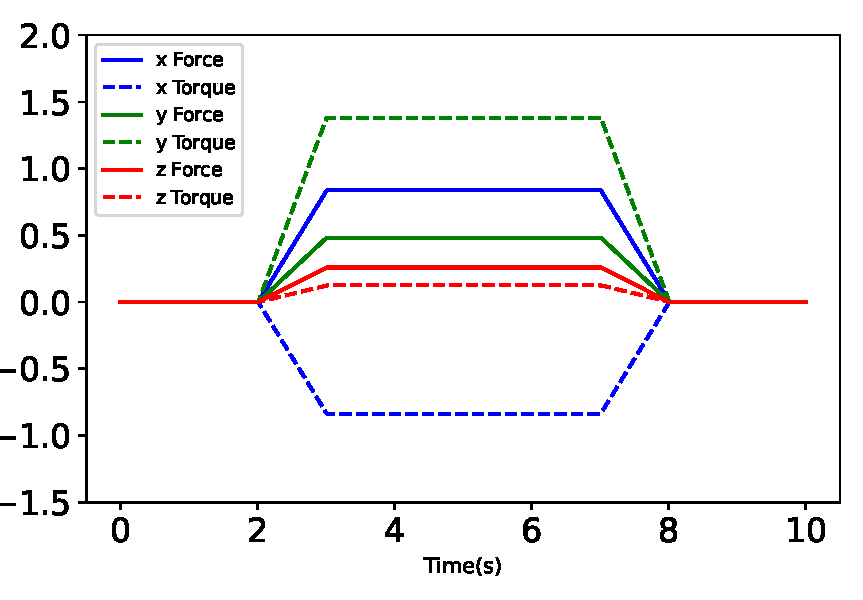
\includegraphics[width=0.8\textwidth]{AutoTeX/Ramp_10steps_CutoffOFF_5s_testRate100}}\caption{All Forces and Torques with 10 step Ramp, thrust for 5s. Cutoff OFF, testRate100}\label{fig:Ramp_10steps_CutoffOFF_5s_testRate100}\end{figure}
	
	As Figure \ref{fig:Ramp_10steps_CutoffOFF_5s_testRate100} shows, the desired behavior is captured exactly for each 
	firing in the test for all of the forces and torques. This is validated by the exact same predicted and simulated thrust arrays. 
	
	\item{\underline{Cutoff firing:}}
	
	We test the ramped thrust with 10 incremental steps. The single thruster is set at the default 30$^\circ$ off the x-axis 15$^\circ$ off the z-axis, at $\bm r = \left(1.125,0.5,2.0\right)$. The thrust is set for 5.0 seconds with a test rate of 10 steps per second. The Cutoff test is ON
	
	Using the same ramp, we start firing the thruster with an initial command of 5 seconds. After just $0.2$ seconds of thrust ramping, we change the test command and thrust for $0.3$ seconds. This leads to a total thrust of $0.5$ seconds, and validates the fact that the command was properly overridden.
	
	\begin{figure}[htbp]\centerline{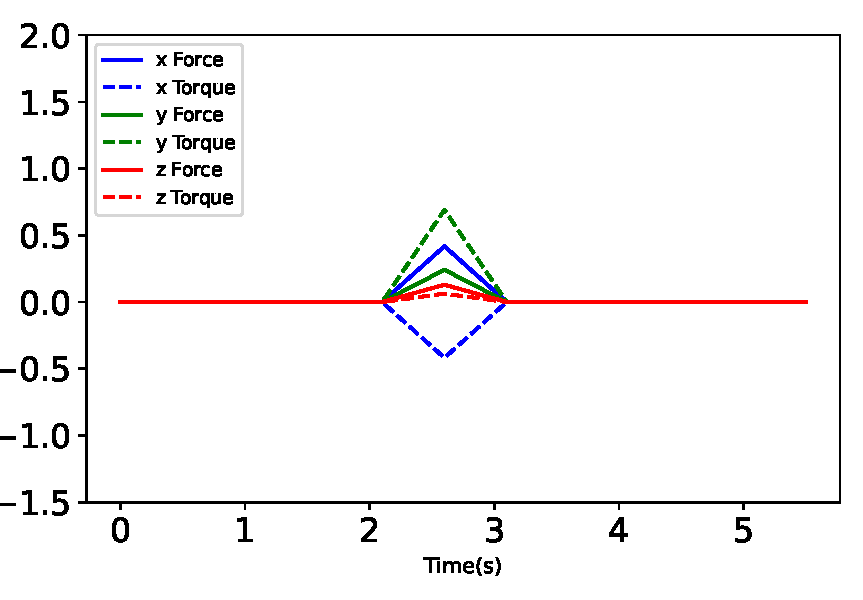
\includegraphics[width=0.8\textwidth]{AutoTeX/Ramp_10steps_CutoffON_5s_testRate10}}\caption{All Forces and Torques, with a 10 step Ramp, thrust for 5s. Cutoff ON, testRate10}\label{fig:Ramp_10steps_CutoffON_5s_testRate10}\end{figure}
	
	As Figure \ref{fig:Ramp_10steps_CutoffON_5s_testRate10} shows, the desired behavior is captured exactly for each 
	firing in the test for all of the forces and torques. This is validated by the exact same predicted and simulated thrust arrays. 
	
	\item{\underline{Ramp down firing:}}
	
	We test the ramped thrust with 10 incremental steps. The single thruster is set at the default 30$^\circ$ off the x-axis 15$^\circ$ off the z-axis, at $\bm r = \left(1.125,0.5,2.0\right)$. The thrust is set for 0.5 seconds initially with a test rate of 10 steps per second. The Cutoff test is ON the RampDown test is ON.
	
	In this test, the initial command is of $0.5$ seconds. On the falling side of the ramp, a new command is given for $1.5$s. We expect to see the thrust climb again to steady state and last for the expected command time.   
	
	\begin{figure}[htbp]\centerline{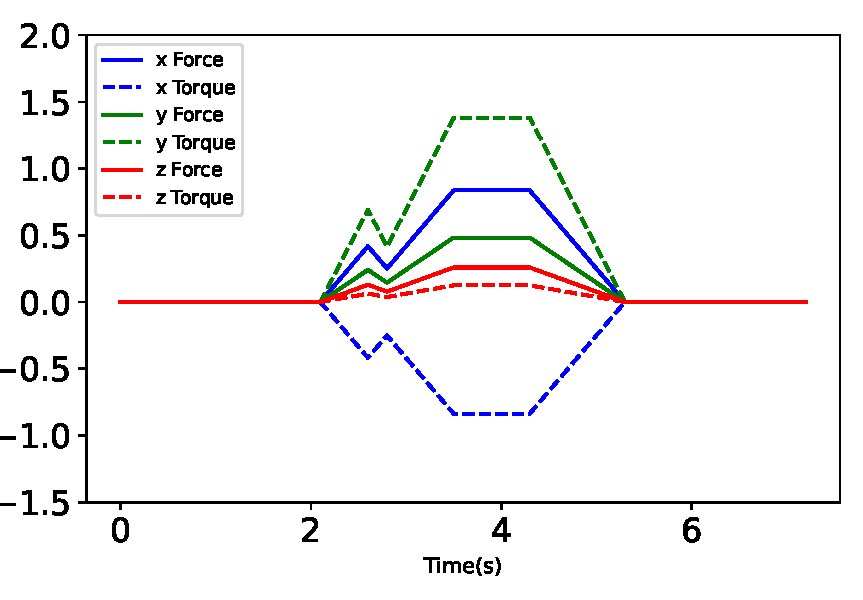
\includegraphics[width=0.8\textwidth]{AutoTeX/Ramp_10steps_CutoffONrampDownON_testRate10}}\caption{All Forces and Torques, with a 10 step Ramp, Cutoff ON, RampDownON testRate10}\label{fig:Ramp_10steps_CutoffONrampDownON_testRate10}\end{figure}
	
	As Figure \ref{fig:Ramp_10steps_CutoffONrampDownON_testRate10} shows, the desired behavior is captured exactly for each 
	firing in the test for all of the forces and torques. This is validated by the exact same predicted and simulated thrust arrays.  
	
\end{enumerate}




\subsection{Test Coverage}
The method coverage for all of the methods included in the spice\_interface 
module are tabulated in Table~\ref{tab:cov_met}

\begin{table}[htbp]
	\caption{Test Analysis Results}
	\label{tab:cov_met}
	\centering \fontsize{10}{10}\selectfont
	\begin{tabular}{c | r | r | r} % Column formatting, 
		\hline
		Method Name    & Unit Test Coverage (\%) & Runtime Self (\%) & Runtime Children (\%) \\
		\hline
		SelfInit & 100.0 & 0.0 & 0.0 \\
		AddThruster & 100.0 & 0.0 & 0.0 \\
		UpdateState & 100.0 & 0.0 & 0.0 \\
		WriteOutputMessages & 100.0 & 0.0 & 0.0 \\
		ReadInputs & 100.0 & 0.0 & 0.0 \\
		ConfigureThrustRequests & 100.0 & 0.0 & 0.0 \\
		ComputeDynamics & 100.0 & 0.0 & 9.8 \\
		ComputeThrusterFire & 100.0 & 0.0 & 0.0 \\
		ComputeThrusterShut & 100.0 & 0.0 & 0.0 \\
		updateMassProperties & 100.0 & 0.0 & 0.6 \\
		\hline
	\end{tabular}
\end{table}

For all of the methods in the spice\_interface modules, the code coverage 
percentage is 100\% which meets our test requirements.  Additionally, 100\% of 
all code branches in the thruster\_dynamics source code were executed by this 
test.

%The test that was run to calculate thruster CPU usage was deliberately selected as 
%a stressing case for the thruster model.  The MOI burn was executed 9000 seconds 
%after the simulation was initialized and that maneuver takes 2000 seconds, so 
%approximately 20\% of the simulation was run with the vehicle under thrust.  
%With this stressing case, the ThrusterDynamics model accounted for 10\% of the 
%overall processing, which is certainly acceptable at this time.

The main CPU usage of the thruster\_dynamics source code occurs in the 
ComputeDynamics method that is called by the dynamics source.  The 
ThrusterDynamics methods themselves account for very little of the processing 
and it is the vector/matrix manipulation utilities called from the source that 
are the main culprits.  While the thruster model's ComputeDynamics function is 
using 50\% of the dynamics processing, that is only amounting to 10\% of the 
overall simulation processing.  The rest of the architecture in Basilisk should 
allow us to take the processing hit that we are getting from the 
ThrusterDynamics module without issue.

\subsection{Conclusions}
The thruster module has sufficient fidelity to accomplish the analysis 
that we need to perform thrust maneuvers.  All model capabilities were 
tested and analyzed in this document with all observed performance being nominal 
compared to the going-in expectation. Every line of source code was successfully tested and the integrated model 
performance was analyzed and is acceptable. Furthermore many thrust scenarios were tested in order to cover all outcomes of a maneuver and the robustness of the simulation.



